\documentclass[xetex,mathserif,serif]{beamer}

\usepackage[catalan]{babel} % Language 
\usepackage{fontspec}
\usepackage{array} % needed for \arraybackslash
\usepackage{graphicx}
\usepackage{adjustbox} % for \adjincludegraphics

\title{Estudi de la ocupació de les aules de la FIB}
\author{Arnau Canyadell Miquel \and Joan Marcè Igual \and Daniel Ferro González}

\date[Juny 2015] % (optional)
{Presentació del treball}
\subject{Estadística}

\begin{document}
  
  \frame{\titlepage}
  
  \begin{frame}{Objectiu}
    \begin{itemize}
      \item Comparar la disponibilitat d'ordinadors entre aules de la FIB on hi ha classe i aules on no n'hi ha.
      \item Comprovar si és cert que \emph{en les aules on hi ha classe la disponibilitat és superior que en les que hi ha classe}.
    \end{itemize}
  \end{frame}
  
  \begin{frame}{Metodologia (1 de 2)}
    \begin{block}{Recollida de dades}
      Obtenció de les dades a través de l'API del Racó de la FIB utilitzant un servidor.
      Informació obtinguda: horaris de les classes i número d'ordinadors lliures / aula.
      \url{https://github.com/jmigual/peFIB}
    \end{block}
    
    \begin{block}{Variables d'estudi}
      \emph{X} = proporció d'ordinadors lliures en les aules on \emph{hi ha classe}.
      \emph{Y} = proporció d'ordinadors lliures en les aules on \emph{no hi ha classe}.
    \end{block}
    
    \begin{block}{Contrast d'hipòtesis}
      $$H_0: \mu_x = \mu_y$$
      $$H_1: \mu_x \neq \mu_y$$
    \end{block}
  \end{frame}

  \begin{frame}{Metodologia (2 de 2)}
    \begin{block}{Premisses}
      \begin{itemize}
        \item $X,Y \sim N$ degut a la seva grandària.
        \item Suposem $X$ i $Y$ independents.
      \end{itemize}
    \end{block}
    
    \begin{block}{Estadístic}
      $$\hat{z} = \frac{\bar{x} - \bar{y}}{\sqrt{s_x^2/n_x + s_y^2/n_y}} $$
      $$\hat{z} \sim N(0,1)$$
      \centering
      Rebutjar si $|\hat{z}| > z_{1 - \alpha/2}$ amb $\alpha = 5\%$.
    \end{block}
  \end{frame}
  
  \begin{frame}{Resultats (1 de 3)}
    \begin{columns}[T]
    \begin{column}{0.4\linewidth}
      \begin{figure}
      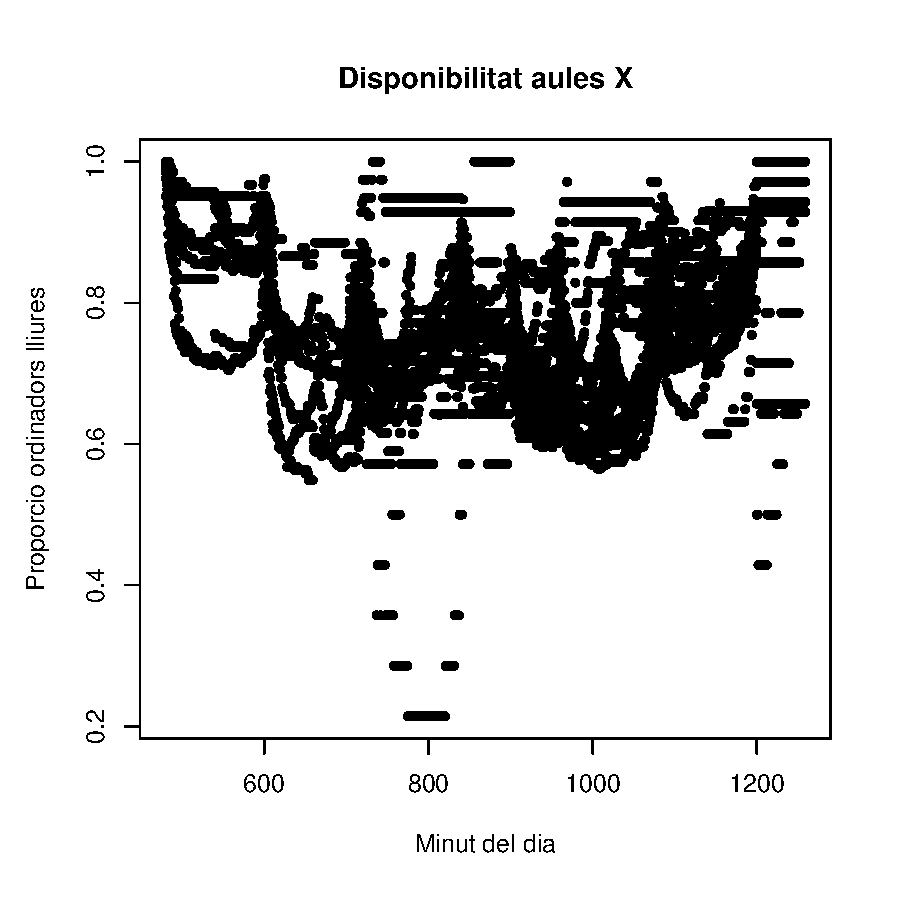
\includegraphics[width=1\linewidth]{./images/dades_X.eps}
      \end{figure}
    \end{column}
    \begin{column}{0.4\linewidth}
      \begin{figure}
      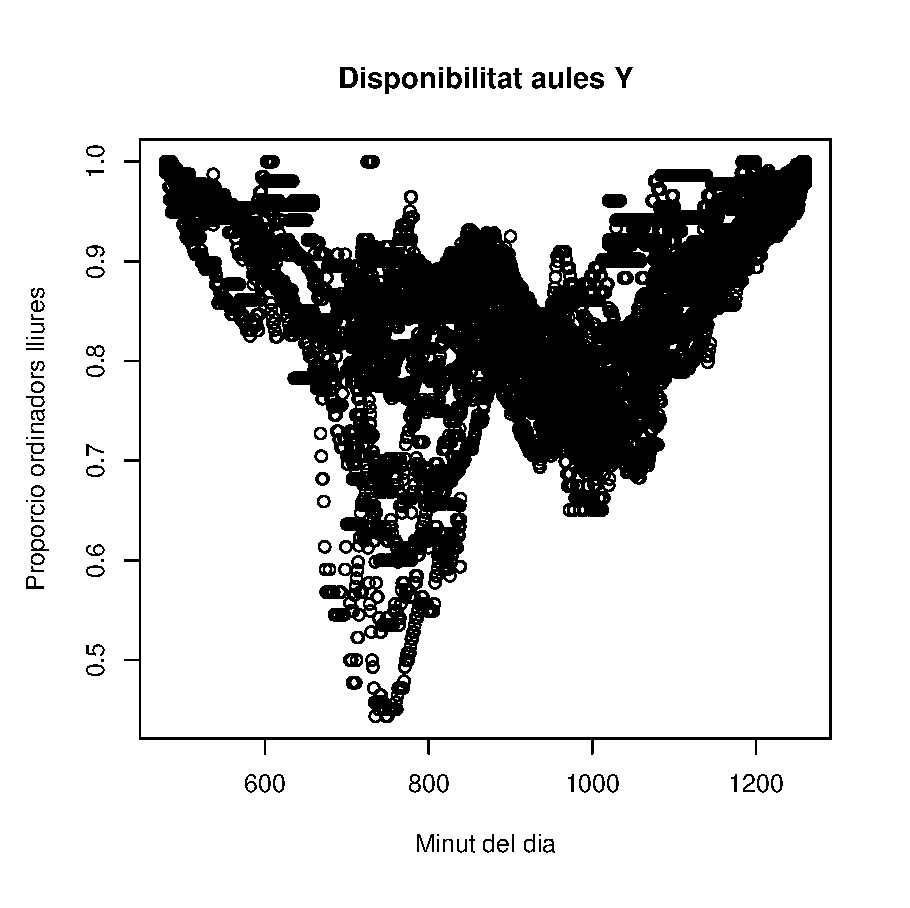
\includegraphics[width=1\linewidth]{./images/dades_Y.eps}
      \end{figure}
    \end{column}
    \end{columns}
    \url{https://docs.google.com/spreadsheets/d/1elGJjdaar26Jyu9gmvHlC1y-p9IX4dDBx0xu2t6Q0hw/pubhtml}
  \end{frame}
  
  \begin{frame}{Resultats (2 de 3)}
    \begin{columns}[T]
    \begin{column}{0.4\linewidth}
      \begin{figure}
      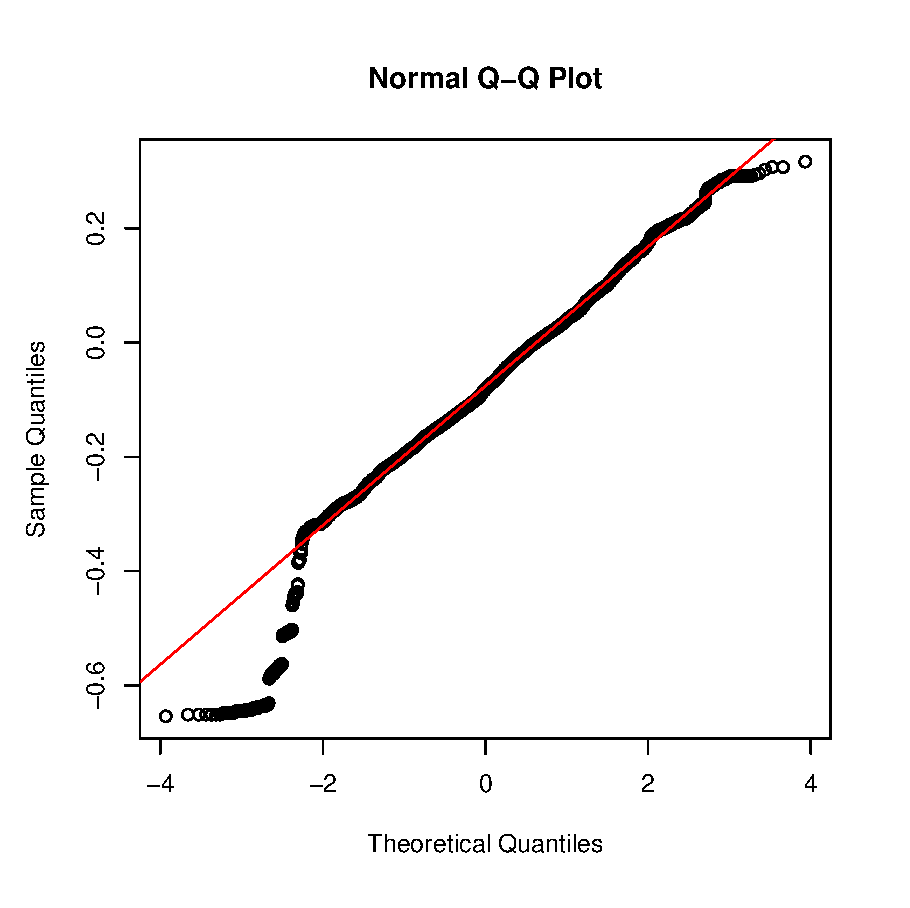
\includegraphics[width=1\linewidth]{images/qqplot}
      \end{figure}
    \end{column}
    \begin{column}{0.4\linewidth}
      \begin{figure}
      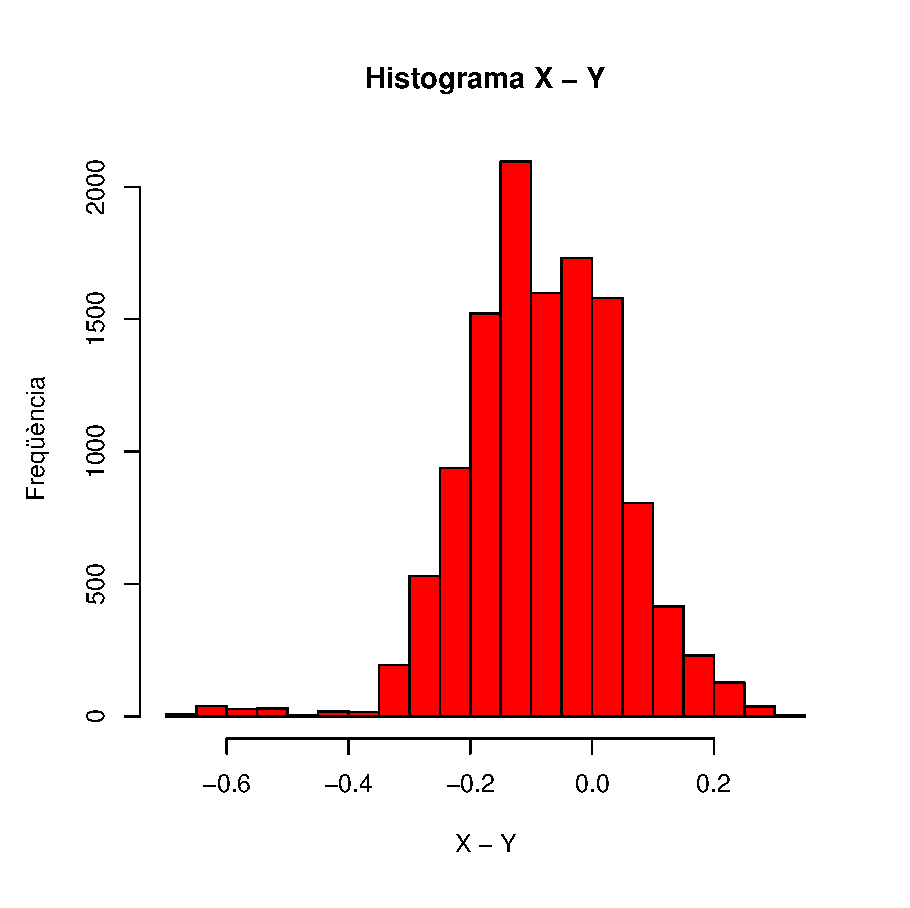
\includegraphics[width=1\linewidth]{images/histograma}
      \end{figure}
    \end{column}
    \end{columns}
  \end{frame}
  
  \begin{frame}{Resultats (3 de 3)}
    $$\bar{x} = 0.77083, s^2_x = 0.01459139, n_x = 11934$$
    $$\bar{y} = 0.8503347, s^2_y = 0.009507904, n_y = 11950$$
    I per tant:
    $$\hat{z} = -55.96263$$
    El p-valor de $\hat{z}$ calculat amb R és 0. Rebutgem $H_0$ i arribem a la conclusió que $\mu_y > \mu_x$
  \end{frame}
  
  \begin{frame}{Discussió}
    La hipòtesi inicial del treball ``\emph{en les aules on hi ha classe la disponibilitat és superior que en les que hi ha classe}'' ha resultat ser falsa. \\
    Atribuïm aquest fet a que hi ha molt poques classes en hores poc concorregudes, sobretot al vespre, que no havíem tingut en compte.
  \end{frame}
\end{document}